\documentclass[a4paper]{article}

\usepackage{INTERSPEECH2019}
\usepackage{multirow}

\title{Multimodal Word Discovery and Retrieval with Phone Sequence and Image Concepts}
\name{Liming Wang$^1$, Mark Hasegawa-Johnson$^{1,2}$}
%The maximum number of authors in the author list is twenty. If the number of contributing authors is more than twenty, they should be listed in a footnote or in acknowledgement section, as appropriate.
\address{
  $^1$Department of Electrical and Computer Engineering, University of Illinois, Urbana Champaign\\
  $^2$Beckman Institute, University of Illinois, Urbana Champaign}
\email{lwang114@illinois.edu, jhasegaw@illinois.edu}

\begin{document}

\maketitle
% 
\begin{abstract}
  This paper demonstrates three different systems capable of performing the multimodal word discovery task.  A multimodal word discovery system accepts, as input, a database of spoken descriptions of images (or a set of corresponding phone transcripts), and learns a lexicon which is a mapping from phone strings to their associated image concepts.  Three systems are demonstrated: one based on a statistical machine translation (SMT) model, two based on neural machine translation (NMT).  On Flickr8k, the SMT-based model performs much better than the NMT-based one, achieving a 49.6\% F1 score. Finally, we apply our word discovery system to the task of image retrieval and achieve 29.1\% recall@10 on the standard 1000-image Flickr8k tests set. 
\end{abstract}
\noindent\textbf{Index Terms}: unsupervised spoken word segmentation, multimodal learning, neural machine translation, statistical machine translation

\section{Introduction}
The task of word discovery is to segment and cluster speech or phone sequences into sequence of word units. It is useful for speech technology for unwritten languages and for languages in which obtaining word segmentation and lexicon manually will be prohibitively expensive.  Automatic word discovery systems exist (e.g.,~\cite{Rasanen2015,Bharadwaj2013,Kamper2017}), but the task is quite challenging, therefore we employ an 
%Since the task has been shown to be quite challenging when using raw speech signal, we propose a two-step process for word unit discovery: first, the raw speech is converted into phonetic sequences, which are much easier to obtain than word boundaries; next, the word boundaries are predicted in an unsupervised fashion from phone sequences. To facilitate the second step, we employ a 
alternative source of information: images.
If each utterance is known to be a spoken description of an image, then the set of concepts visible in the image can be seen as a bag of noisy word labels for the speech.
%where only the type of words in the caption is available but not the positions of them.

%\section{Related Works}
Several works have used raw audio to discover word units.
%Besides cognitive-driven and heuristic-based methods aiming to find certain
Methods that imitate child language acquisition often begin by finding
recurring patterns in audio \cite{Rasanen2015,Park2008}.
Non-parametric Bayesian hidden Markov models (HMMs) have been widely used in word-unit discovery and various other clustering problem with audio,
e.g., a latent Dirichlet process with HMM acoustic models can be used to jointly segment and cluster raw audio into sub-word units~\cite{Lee2012,Ondel2018},
or the HMM can be regularized using an
L-p norm as sparsity constraint to encourage purer clusters\cite{Bharadwaj2013}.
%For word discovery, \cite{Kamper2017} used acoustic
Using word embeddings as features, it is possible to perform automatic word discovery by modeling each word as a Gaussian mixture model with a Dirichlet prior on its parameters; the model can be trained using expectation maximization (EM), or using a weighted K-means algorithm~\cite{Kamper2017}.
The Dirichlet-prior Gaussian mixture model out-performed all other systems by around 10 \% (30 \% in F-score) during the 2017 zero-resource challenge \cite{Dunbar2017}.
Other works have focused on discovering word units from phone sequences or character sequences, such as models based on Pitman-Yor process \cite{Johnson2007}.  

A related task to the unsupervised spoken word discovery is query-by-example keyword search in audio, which aims to only search for a collection of keywords and leaves the rest of the speech as background.
%Several systems has reported results on the benchmark for the task,
The most recent widely published benchmark evaluation of this task was the
NIST OpenKWS evaluation set on the language Georgian.
The Kaldi OpenKWS system \cite{Trmal2017} trained a DNN-HMM hybrid system and decode the OOV queries by fusing the decoding scores on word-level (with proxy word), phonetic-level and morpheme-level lattices to maximize the ATWV score.
The BBN system \cite{Alumae16} combined several acoustic models based on DNN, LSTM and CNN on subword units to perform joint decoding and handled OOV queries on the sub-word unit.
The STC keyword search system \cite{Medennikov2017} combined 9 different acoustic models based on DNN and GMM with a phone-posterior based OOV decoder \cite{Khokhlov2017}.  

A multilingual approach for spoken word discovery has been proposed by \cite{Stahlberg12}, who developed a variant of the IBM model 3 SMT to discover word units of an under-resourced language
by aligning parallel texts in
%with transcriptions of
a high-resourced language.
%\cite{Duong16} first proposed the use of
The same task has been attempted~\cite{Duong16} using NMT with attention \cite{Bahdanau14} to align speech or phone sequences to the word labels of the high-resourced language; modifications of the attention mechanism to ensure coverage and richer context.
If the true phone sequence in the under-resourced language is unknown,  pseudo-phone labels generated by an unsupervised non-parametric Bayesian model \cite{Ondel2018} can be used as input to the NMT~\cite{Godard2018}.
 
%Other works have been done on discovering semantic units via multimodal learning of natural language and image  \cite{Hodosh2010}\cite{Harwath15}\cite{Harwath16-ULO}\cite{Harwath17}.
The database used in this paper was first published as an image captioning corpus, for which the baseline system
\cite{Hodosh2010} used IBM model I and II \cite{Brown93} combined with Kernel Canonical Component Analysis (KCCA) for mapping both image and text to a joint space. \cite{Karpathy14, Karpathy15} developed a two-branch neural network system to learn the joint representation of image and text.
%\cite{Harwath15}\cite{Harwath16-ULO}\cite{Harwath17} discovered the semantic units with audio and image after training an end-to-end retrieval system.
The speech files were first used to train an end-to-end image retrieval system~\cite{Harwath15,Harwath16-ULO}, and were then further analyzed to discover word-like units~\cite{Harwath17}.
The task of multimodal word discovery was, we believe, first proposed in~\cite{Harwath17}, where it was performed as a generalization of the image retrieval problem: every possible subsegment of the audio file was tested as a query, and every possible sub-region of the image was tested as a possible retrieval result.

\section{Problem formulation}
\subsection{Word discovery as neural machine translation}
Suppose we have a sequence of phone indices $x_1, ..., x_{T_x}$ and a sequence of image concepts $y_1, ..., y_{T_y}$, where $x \in \mathcal X, y \in \mathcal Y\cup \{NULL\}$.
Given $(\mathbf{x}, \mathbf y)$, the goal of our algorithm is a sequence learning problem to align each phone label $\mathbf{x} = [x_1, x_2, \ldots, x_{T_x}]$ to an image concept $\mathbf{y} = [y_1, y_2, \ldots, y_{T_y}]$.
We assume that $T_y < T_x$ and one phone label is only associated with one or none of the image concepts.
In other words, we define an alignment matrix $\mathbf A \in \{0, 1\}^{T_y  \times T_x}, \mathbf{A} = [\mathbf{a}_1 \ldots \mathbf{a}_{T_x}] = [\tilde{\mathbf a}_1^{\top} \ldots \tilde{\mathbf a}_{T_y}^{\top}]^\top$, and we have:
\begin{align}\label{eq:cluster_constraint}
\sum_{i=1}^{T_y} a_{it} = 1, \forall t \in \{1, \ldots, T_x\}.
\end{align}
Then our model tries to learn to maximize:
\begin{align}\label{eq:trans_prob}
    p(\mathbf{y}|\mathbf{x}) = \sum_{\mathbf{A}\in \{0, 1\}^{T_y  \times T_x}} p(\mathbf{A}|\mathbf{x}) p(\mathbf{y}|\mathbf{x}, \mathbf{A}),
\end{align}
for each input phone-concept sequence pair. 
%\begin{figure}
%    \centering
%    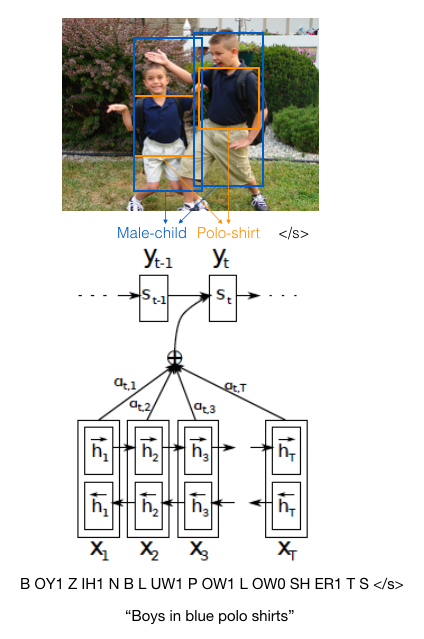
\includegraphics[width=0.3\textwidth]{submission/fig_1.png}
%    \caption{Attention-based Word Discoverer}
%    \label{fig:nmt_model}
%\end{figure}

Suppose there is a ``dominant alignment'' $\mathbf{A}^*$such that $p(\mathbf{A}^*|\mathbf{x})\approx 1$, Eq.~(\ref{eq:trans_prob}) is then simplified to one term:
\begin{align}\label{eq:trans_prob_dominant}
     &p(\mathbf{y}|\mathbf{x})
     \approx p(\mathbf{y}|\mathbf{x}, \mathbf{A}^*)  \approx
     \prod_{i=1}^{T_y} p(y_i|y_{1:(i-1)},\mathbf{x}, \mathbf{A}^*).
%     \approx p(\mathbf{A}|\mathbf{x}) p(\mathbf{y}|\mathbf{x}, \mathbf{a}^*)  \approx p(\mathbf{y}|\mathbf{x}, \mathbf{a}^*).
\end{align}
where $y_{1:(i-1)}=[y_1,\ldots,y_{i-1}]$ is the set of output labels preceding $y_i$.
Another simplification we can make is to compress the one-hot representations of the phone sequence $\mathbf{x}_i, i=1,...,T_x$ into a lower-dimensional embedding vector $\mathbf{h}_i, i=1,...,T_x$ and learn the dominant alignment with a soft alignment:
\begin{align}\label{eq:attention}
    a^*_{it} &:= \mathbf\alpha_{it} =  \frac{\exp(e_i(\mathbf h(\mathbf x_t), \mathbf s_{i-1})/T)}{\sum_{j=1}^{T_y} \exp(e_j(\mathbf h(\mathbf{x}_t), \mathbf s_{j-1})/T)}\\
    \mathbf{c}_i &= \sum_{t=1}^{T_x} a^*_{it} \mathbf{h}_{t},
\end{align}
where $\mathbf e(\cdot)$ can be learned by a neural network,
$\mathbf{s}_i$ is the decoder state vector, and 
$\mathbf{c}_i$ is called the \textit{context vector} in a typical encoder-decoder architecture \cite{Bahdanau14}.
$T$ is a temperature term to smooth the softmax \cite{Duong16}.
%Let $\mathcal C_i, i=\{1,...,|\mathcal Y|\}$ be the corresponding cluster of phone indices of a given image concept, we assume then $\mathbf{y}_i$ is independent of $x_j, j\not\in \mathcal C_i$ and dependent on $x_j, j\in \mathcal C_i$ only through $c_i$.
A main difference of
our network from the architecture in \cite{Bahdanau14} is that instead of normalizing the energy over the time steps of the input phone sequence, our network normalizes across the attention weights corresponding to the output image concepts for each phone. This helps ensure the assumption in Eq. (\ref{eq:cluster_constraint}) is satisfied and our alignment for each phone is sparse across image concepts.
Let us further assume that $y_i$ depends on $\mathbf{x}$ only by way of its dependence on $\mathbf{c}_i$,
and depends on $y_{1:(i-1)}$ only by depending on $y_{i-1}$ and $\mathbf{s}_{i-1}$, therefore
%Plug Eq. (\ref{eq:attention}) into Eq. (\ref{eq:trans_prob_dominant}):
\begin{align}
    \prod_{i=1}^{T_y} p(y_i|y_{1:i-1}, \mathbf{x}, \mathbf{A}^*) \approx
    \prod_{i=1}^{T_y} p(y_i|y_{i-1}, \mathbf{s}_{i-1}, \mathbf{c}_i).
%    \prod_{i=1}^{T_y} p(y_i|y_{1:i-1}, \mathbf{x}, \mathbf{a}^*) \approx
%    \prod_{i=1}^{T_y} p(y_i|y_{i-1}, \mathbf{s}_{i-1}, \mathbf{c}_i).
\end{align}
The set of probabilities $\{p(y_i|y_{i-1}, \mathbf{s}_{i-1}, \mathbf{c}_i)\}_{i=1}^{T_y}$ can be learned using a recurrent neural net $f$ with state vectors $\mathbf{s}_i$. Now the task reduces to learning the functions $h, e, f$ such that the log-likelihood of the concepts given the phone sequence is maximized.

%\begin{figure}
%    \centering
%    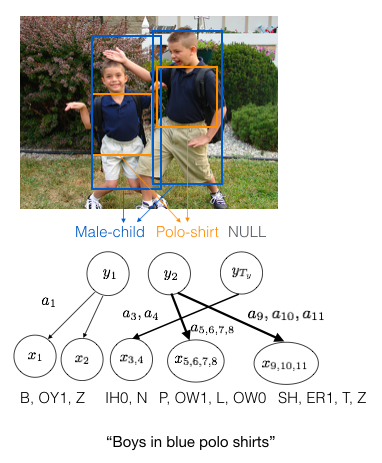
\includegraphics[width=0.3\textwidth]{submission/fig_2.png}
%    \caption{Statistical Word Discoverer}
%    \label{fig:nmt_model}
%\end{figure}

For the neural-based translator, we used XNMT \cite{neubig18xnmt} to implement two networks: One used a standard encoder-decoder structure with attention normalized over the phone sequence, which we will refer to later as the normalized-over-time model;
the other has the same bi-directional LSTM encoder with a single 512-dimensional hidden layer but with attention normalized over the concepts.
The decoder for the normalized-over-concepts model does not have recurrent state operation
(because the state vector $\mathbf{s}_i$ depends on the context vector $\mathbf{c}_i$, which depends on
$\mathbf{s}_j$ for times including $j>i$, as shown in Eq.~\ref{eq:attention}),
%(otherwise, the network will run into cycle: to compute $\alpha_{it}$ $e_{it}$ is required for all $i$ but to compute $e_{i't}, i'>i$, $\alpha_{it}$ is required since it is required to the context vector $c_{i'}$), and
instead, the concept label is fed into the attention network. The attention networks for both models have a single 512-dimensional hidden layer.

\subsection{Word discovery as statistical machine translation}
Alternatively, we can learn the probability of a phone sequence given a set of image concepts:
\begin{align}\label{eq:smt_trans_prob}
    p(\mathbf{x}|\mathbf y) &= \sum_{a_1 = 0}^{T_y} \sum_{a_2 = 0}^{T_y}\ldots \sum_{a_{T_x} = 0}^{T_y} p(\mathbf{A}|\mathbf y)p(\mathbf x |\mathbf y, \mathbf{A}).
\end{align}
Following \cite{Brown92}, we make use of the following assumptions: 1)
$\mathbf{A}$ is integer-valued, specifically $a_{it}=1$ for $i=i(t)$, else $a_{it}=0$,
2) all alignments are equally likely given only $\mathbf{y}$: $p(\mathbf A|\mathbf y) = \frac{\epsilon}{(T_y+1)^{T_x}}$, where $\epsilon$ is some normalization constant;
3) given the alignment,
%$\forall y_j, j\neq a_i$ is conditionally independent of $x_i$ and $x_i$'s are independent of $x_j, j\neq i$ given $y_{a_i}$:$p( \mathbf{x}|\mathbf{y}, \mathbf{a}) = \prod_{i=1}^{T_x} p(x_i|x_{1:i-1}, y_{a_i}) = p(x_i|y_{a_i})$.
each phone depends only on its aligned image concept, thus
$p(x_t|x_{1:(t-1)},\mathbf{A},\mathbf{y})=p(x_t|y_{i(t)})$.
Eq. (\ref{eq:smt_trans_prob}) is then simplified to:
\begin{align}
%    &\frac{\epsilon}{(T_y+1)^{T_x}}\sum_{a_1 = 0}^{T_y} \sum_{a_2 = 0}^{T_y}\ldots \sum_{a_{T_x} = 0}^{T_y} 
%    \prod_{i=n}^{T_x}p(x_i|y_{a_i}).
    &\frac{\epsilon}{(T_y+1)^{T_x}}\prod_{t=1}^{T_x}\sum_{i(t)=1}^{T_y} p(x_t|y_{i(t)}).
\end{align}
Optimization with EM results in 
%which can be optimized with EM algorithm and result in
an iterative formula
 in terms of the expected counts of a given phone-concept pattern.

The optimal alignment between the phones and image concepts can be then obtained by finding the highest-scored translation pair of a given sentence:
\begin{align}\label{eq:smt_alignment}
    i^*(t) = \arg\max_i p(x_t|y_i).
\end{align}

%\subsection{Model Description}
%\subsection{Image Retrieval}
%To tackle the translation formulation of the word discovery problem, we will employ two types of models: A neural-based translation model described in \cite{Bahdanau14} and a statistical translation model based on \cite{Brown93}.

To perform image retrieval using the SMT model, for each image example we compute the translation probability of the phone sequence given the image concepts: $P(\mathbf x|\mathbf y)$.
For phone-translation pairs unseen before, we simply filled in for the pair a small fixed probability $10^{-12}$.

\section{Experimental setup}
\subsection{Datasets}
%We used the flickr8k dataset \cite{Hodosh2010} for both word discovery and image retrieval. The dataset contains 8000 images and 5 captions per image. We selected a subset of the caption that contains the exact phrase in the phrasal labels of the bounding boxes, which includes 7996 images with one caption per image and 20621 annotated word phrases in the subset. For the retrieval, we split the dataset to have the same test set of 1000 images as in  
%\cite{Karpathy14}\cite{Harwath15}, but we did not use a validation set. 

Our dataset consists of 7996 images that are present in both the Flickr8k~\cite{Hodosh2010} and Flickr30k corpora.
We used the Flickr30kEntities dataset to extract the image concepts and phone sequences primarily because it contains bounding boxes with phrases from the caption that describes the particular region, like ``a girl in a white shirt''.
The phrase-level segmentation is used as our groundtruth alignments.
Only the images
that also
appeared in Flickr8k are used,
so that we can compare our results to 
%for comparison with
other speech-to-image~\cite{Harwath15} and text-to-image~\cite{Karpathy14} retrieval systems.
%models like \cite{Harwath15}.
In order to make sure that our image retrieval results use the same dataset as~\cite{Harwath17}
and~\cite{Karpathy14}, we divided the data into a training set
(6996 images) and a test set (the same 1000 images that are used as the test set
in~\cite{Harwath17,Karpathy14}).
%Also we
For word discovery, we 
restricted our attention to a list of concepts that appeared at least 10 times in our training dataset.
By using the WordNet~\cite{Miller1995} synsets to merge similar concepts, we were
able to find a list of 1547 distinct image concepts, each of which occurs at least 10 times.
%and created a set of 1547 image concepts using Wordnet synsets \cite{Miller1995}.
We merged repeated concepts in a sentence in order to maintain the many-to-one mapping between the phone sequence to concept.
The captions are converted into phone sequences via the CMU pronunciation dictionary \cite{Rudnicky2014}, which contains 39 distinct phonetic symbols and 69 symbols in total with the stress symbol. Compound words such as ``fingerpaint'' or ``skateboarder'' do not have an entry in the dictionary, and we simply replace them with an \texttt{UNK} symbol.
We used NLTK \cite{BirdKleinLoper09} as the interface to both Wordnet and CMU dictionary.
Notice that we did not use an image classifier to compute the probabilities of the image concepts and instead used the hard label from Wordnet because we believe the task of detecting the image label is largely separate from our main task;
%, as we can train a separate network pretrained on a large amount of data to detect the image concepts and then train our system with the predicted image labels and phone sequences. It will leave as our future work
future work will seek
to integrate such an image classifier into our system. 

\subsection{Evaluation metrics}
For the word discovery task, we evaluated our results by comparing the predicted alignment with the groundtruth.
Several metrics are used to evaluate the system:
The word intersection-over-union (IoU) measures
the similarity between the span of a discovered phone sequence and the span of the
groundtruth image concept at the same location in the phone string
%how close is the learnt units to a word
by measuring the ratio of the length of their intersection, divided by the length of their union.
%of the ground-truth words and the closest
%predicted words in term of position in the sentence. We measure the accuracy of the model detecting the correct alignment.
Accuracy is measured as the percentage of phones that are assigned to the correct image concept.
To visualize the tradeoff between the true positive rate and false positive rate, we also plot the receiver operating characteristic (ROC) curve using the alignment probability for the SMT and the attention weights for the NMT for each class.
The ROC is defined by treating 
%Alternatively, we treat
the word discovery as a retrieval problem where the query is an image concept and the retrieved documents are the relevant words;
using this setup we 
measure the recall, precision and F-measure of the system. This helps us to fairly evaluate the system because our dataset is unbalanced in amount of instances for each image concept. 
For the image retrieval task, we followed \cite{Harwath15,Karpathy14}
in using recall@1, 5, 10, which treats the entire caption as the query,
and the set of test images as the database.
We also follow~\cite{Harwath15,Karpathy14} in assuming a one-to-one mapping between captions and images,
despite the large number of image pairs with similar concepts. 

%\subsection{Implementation Details}
%For the attention-based model, we used the XNMT \cite{neubig18xnmt} toolkit with standard translator configuration for the normalize-over-time model; for the normalize-over-concept model, we use an attention model with the same input, hidden and output dimension as the normalize-over-time case for fair comparison. Since we do not fine-tune our models, we do not claim our results to represent the optimal performance. 

\section{Results}
%\subsection{Word Discovery Results}

\begin{table}[th]
    \centering
    \caption{SMT vs NMT: Word Discovery Results}
    \begin{tabular}{|c|c|c|c|}
    \hline
        & \multirow{3}{*}{SMT} & NMT  & NMT\\
        & & (norm. over & (norm. over \\
        & & concepts) 	& time)\\
    \hline
    Word-IoU & 6.00 & \textbf{46.0} & 21.0 \\
    Accuracy & \textbf{43.8} & 23.0 & 41.5 \\
    Recall   & \textbf{52.9} & 18.0 & 29.2 \\
    Precision & \textbf{46.7} & 12.1 & 33.0 \\
    F-Measure & \textbf{49.6} & 14.5 & 31.0\\
    \hline
    \end{tabular}
    \label{tab:word_discovery_res}
\end{table}

The word discovery results of our system are shown in Table~\ref{tab:word_discovery_res}.
The SMT model performs the best in almost all the evaluation metrics.
It may be that SMT outperforms NMT
because the size of our dataset ($\approx 100000$ phones and 40000 image concepts) is more suitable for SMT than NMT.
However, we notice that the NMT normalized-over-time has an accuracy
almost equal to that of SMT,
although its recall, precision, and F-measure are low.
The disparity between F-measure and accuracy may indicate that the
disparity between SMT and NMT has less to do with the amount of training data than
with 
%performs almost as well as the SMT given the small amount of data we have in terms of accuracy of alignment.
%For the retrieval-based metrics, SMT performs better (by about 50 $\%$) than NMT,
%suggesting
the imbalanced numbers of training tokens for different image concepts.
%has a bigger impact on the NMT-based model.
For example, the concept with the highest number of groundtruth aligned phones is the
NULL class; it is possible for NMT to achieve high accuracy but low F-score
by simply aligning all phones to the NULL class.
%and the accuracy score of the NMT is inflated by the amounts of true negative phones in the captions.

\begin{figure}[th]
    \centering
    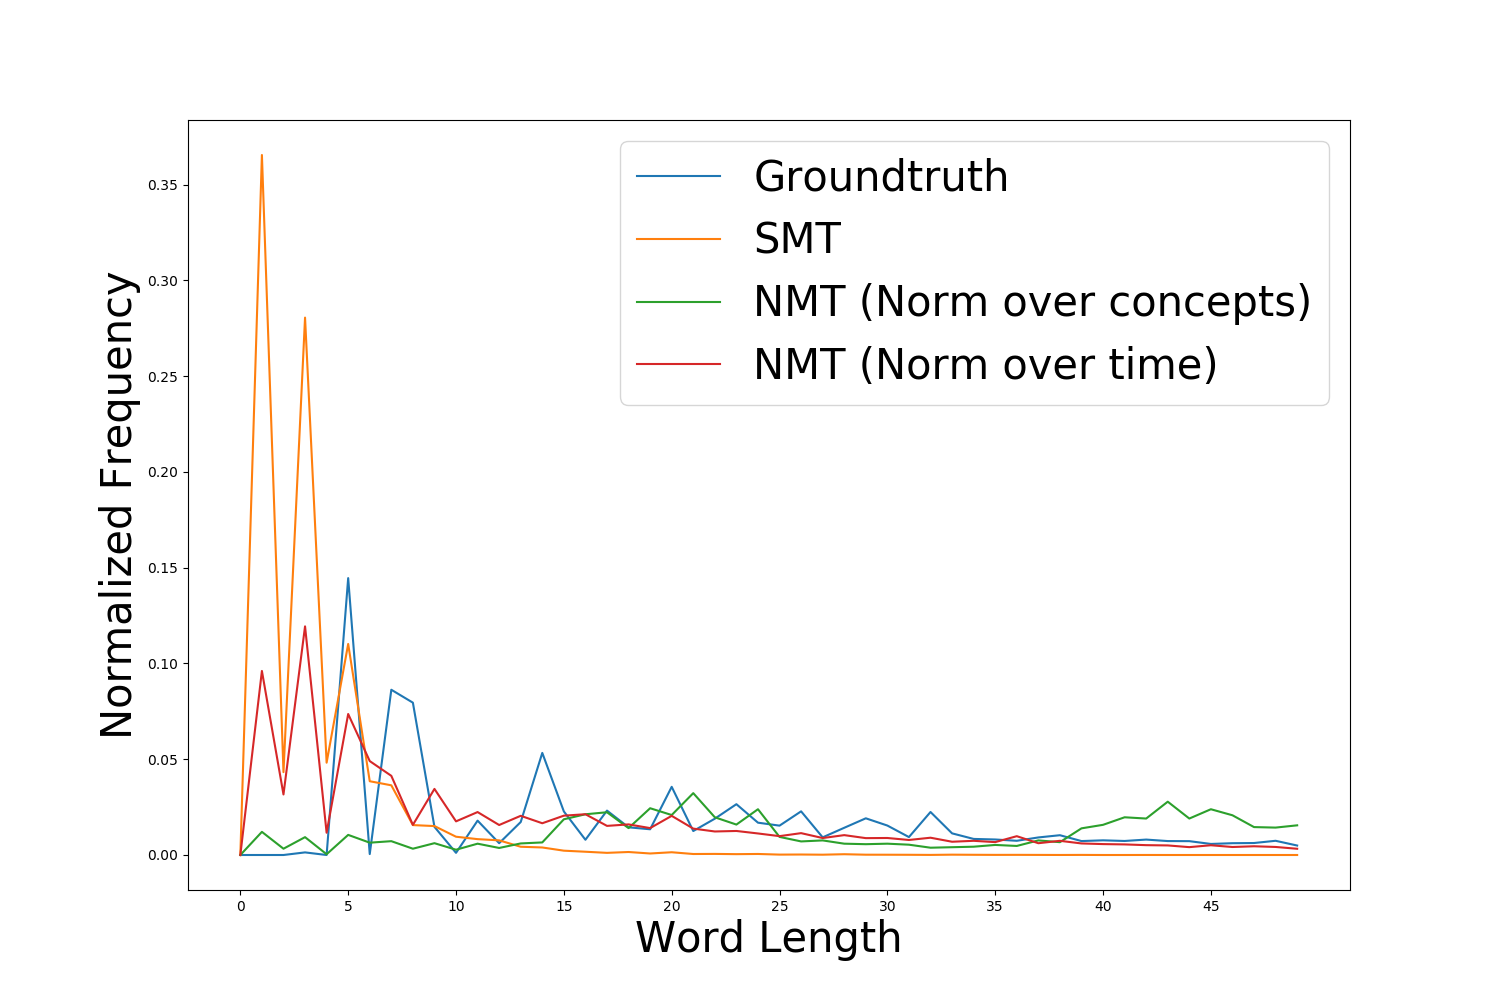
\includegraphics[width=0.5\textwidth]{fig_4.png}
    \caption{Normalized frequency of the lengths of words from the groundtruth and discovered by the models}
    \label{fig:pseudoword-len}
\end{figure}

The NMT generally performs better at IoU scores than the SMT.
A plausible explanation of this finding is
%can be
illustrated in Fig. (\ref{fig:pseudoword-len}): about 40 $\%$ of the pseudo-words discovered by the SMT are less than 3 phones long, and 90 $\%$ of the pseudo-words are within 10 phones long.
%; on the contrary,
By comparison,
the NMT normalized over concepts
tends to generate pseudo-words that are much longer than an actual word, potentially merging various words together. Since the IoU
%tend to bias toward
penalizes 
longer sequences
less than it penalizes shorter sequences, NMT has a higher score than SMT.
The NMT with attention normalized over time seems to have a length distribution closest to the ground truth. 

\begin{figure}[th]
    \centering
    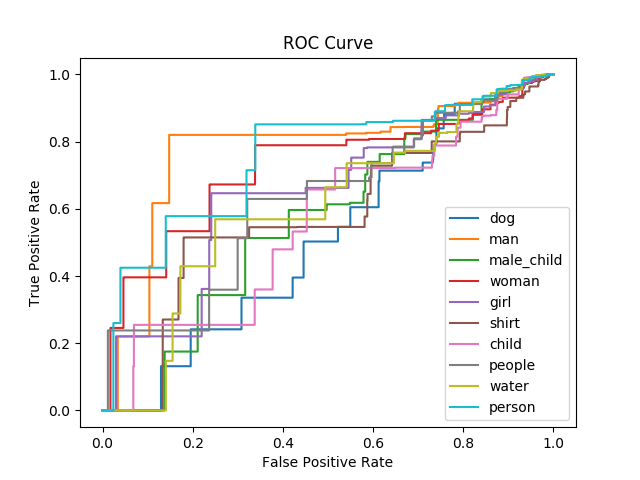
\includegraphics[width=0.5\textwidth]{fig_3.png}
    \caption{ROC curve of the statistical word discoverer for the top-10 concepts (excluding NULL) in the flickr30k dataset}
    \label{fig:smt_roc}
\end{figure}

\begin{figure}[th]
    \centering
    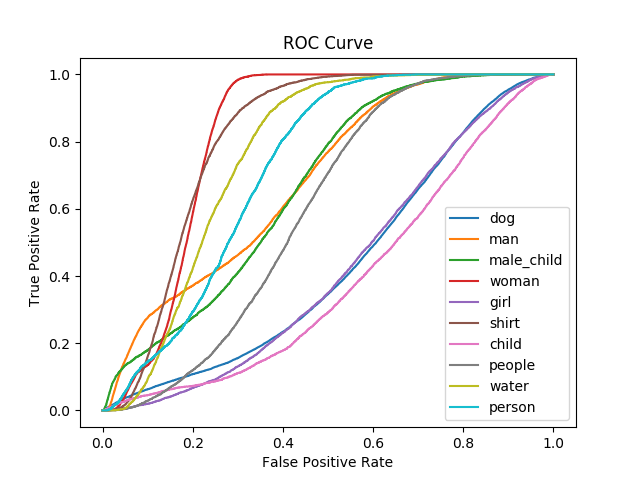
\includegraphics[width=0.5\textwidth]{fig_5.png}
    \caption{ROC curve of the attention-based word discoverer for the top-10 concepts (excluding $<$/s$>$) in the flickr30k dataset}
    \label{fig:nmt_roc}
\end{figure}

The ROC of the SMT and NMT (normalized over time) for the top-10 image concepts is shown respectively in Fig. (\ref{fig:smt_roc}) and Fig.(\ref{fig:nmt_roc}).
These figures show that the SMT is capable of detecting some frequent image concepts,
like ``girl'' or ``man'', accurately with a small false positive rate.
The model, however, fails to control the false positives beyond chance level for the extremely common concept ``dog''.
NMT also has trouble rejecting false positive of the ``dog'' concept,
but seems to be much better at detecting other common concepts such as ``woman'' and ``shirt''.


Between the two NMT models, the normalized-over-time model performs better than the normalized-over-concept model,
even though the normalized-over-time model fails to satisfy Eq.~(\ref{eq:cluster_constraint}).  
%despite the latter is more theoretically appealing.
One explanation may be that the normalized-over-concept model ignores
%the dependency
spatial proximity relationships,
%between various concepts,
such as the tendency for ``hand'' to be visible near ``human'',
since its decoder does not
use the state vector of the decoder network to calculate attention.
%have the recurrent operation between the state in order to accomodate the normalization-over-concept operation.
The difference in performance between the normalized-over-time and normalized-over-concepts models might therefore be interpreted to mean that spatial proximity relationships between image concepts can be useful for multimodal word discovery.
%may help the network to discover word units more efficiently. 

\begin{table}[th]
    \centering
    \caption{Image retrieval rates using SMT multimodal word discovery, compared to speech-based and text-based published results for the same corpus.}
    \begin{tabular}{|c|c|c|c|}
    \hline
             & Recall@1 & Recall@5 & Recall@10\\
             \hline
             SMT & 9.42\% & 21.1\% & 29.1\% \\
         Harwath\&Glass \cite{Harwath15} & - & - & 17.9\% \\
         Karpathy \cite{Karpathy14} &10.3\% &31.4\% & 42.5\%\\
         \hline
    \end{tabular}
    \label{tab:retrieval_res}
\end{table}

%\subsection{Retrieval results}
Image retrieval scores for these systems are shown in Table~\ref{tab:retrieval_res}.
Our SMT system achieves $29 \%$ recall@10 score in a database of 1000 images from Flickr8k.
This is better than the results reported in \cite{Harwath15}, though the comparison is not entirely fair:
We assume the image and phone labels are extracted perfectly, while \cite{Harwath15} does not have such an assumption. Our results are worse than \cite{Karpathy14}, partly because their system is trained on words with known boundaries and on a much larger flickr30k dataset, though they do not assume perfect image labels. Another reason is that our system used only entity labels of the image and no information about the action and pose of the objects in the image is used. The results suggest that our model needs to be extended to incorporate richer context to get higher performance on the retrieval task.

\begin{figure}[th]
    \centering
    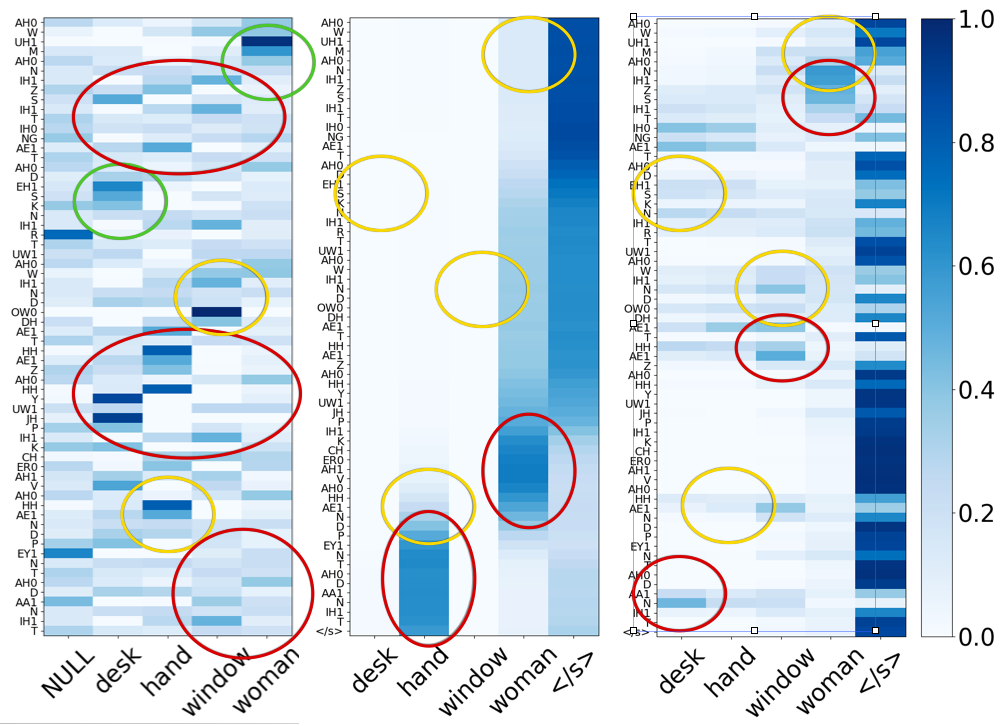
\includegraphics[width=0.5\textwidth]{fig_6_2.png}
    \caption{Comparison of the attention/alignment probabilities for the SMT and NMT models for the caption ``A \textbf{woman} is sitting at a \textbf{desk} near to a \textbf{window} that has a huge picture of a \textbf{hand} painted on it''.  The correctly discovered words are circled in green, the false negative or partially correct words in yellow and the false positive words in red. 1) Left: the SMT model correctly discovers the words ``woman'' and ``desk''  and partially discovered ``hand'' and ``window'', while generating many false positives; 2) Middle: the normalized-over-concept NMT model detects ``woman'' and ``hand'' but is overpowered by the $</$s$>$ symbol; 3) Right: the normalized-over-time NMT model almost correctly discovers the concept ``woman'' and ``window'' but not ``desk'' and ``hand''.}
   % \caption{Comparison of the attention/alignment probabilities for the SMT and NMT models for the caption ``A baby wearing a Santa hat and a red outfit playing with a Santa Claus figure''. The correctly discovered words are circled in green, the false negative words are circled in yellow and the false positive words are circled in red. 1) Left: the alignment probabilities for the SMT model, with each row representing the posterior probability $P(y_j|x_i)$ for a given phone $x_i$. 2) Middle: the attention weights for the normalize-over-concept NMT model; 3) Right: the attention weights for the normalize-over-time NMT model, with each row normalized to one to better visualize the weight distribution for a given phone.}
    \label{fig:attention_compare}
\end{figure}
\section{Error analysis}
%\subsection{Word Discovery}
The attention/alignment matrices of a typical caption is shown in Fig. (\ref{fig:attention_compare}). As shown in the plots,
many of the errors in our systems are caused by the alignment of phones that should belong to the NULL/$</$s$>$ class. 
%(the first column of the leftmost matrix for SMT and the last column for the other two matrices for NMT) to some other image class (the other four columns).
%come from failure of detecting whether a phone actually associates with a image concept or not. A large portion of the false positives of the SMT model are phones belonging to the NULL class.
This may be due to an underestimate of the prior probabilities of the NULL symbol.
Conversely, the NMT tends to overestimate the probability of the end-of-sentence symbol $<$/s$>$,
and therefore it mis-aligns phones that belong to a true concepts to the end symbol.
This example also suggests that
%It also confirms that
the accuracy score of the normalized-over-time model may be inflated by true negative examples,
i.e., by the allocation of phones whose true label should be NULL (the first column of each matrix
in the figure) to other classes.

%\subsection{Image Retrieval}
The main source of error of our image retrieval system is the confusion between images with very similar sets of objects.
This is partly because, unlike \cite{Karpathy14}, our network does not use
a max-margin loss objective,
so the classification boundaries between similar image concepts are not optimally generalizable.
%and trains purely with log-likelihood.
Also richer contexts may be useful to augment the difference between the representation for different images. 

\section{Conclusions}
This paper describes three systems for the 
%In this paper, we present a novel
task of discovering word units from phone labels and image concepts.
%and compare the performance of three baseline models on the task based on statistical machine translation and neural machine translation.
With the amount of data we have, the SMT-based model performs much better than the NMT-based ones, according to our evaluation metrics.
Finally, we applied our word discovery system to the task of image retrieval and show that it can achieve  performance that is about halfway between the published scores for speech-based and text-based image retrieval.

\section{Acknowledgements}
The idea of this work originated from the 2017 JSALT workshop at Carnegie Mellon University, Pittsburgh. We would like to thank \cite{Hodosh2010} for releasing the Flickr8k dataset.

\bibliographystyle{IEEEtran}

\bibliography{sp2019_refs.bib}

% \begin{thebibliography}{9}
% \bibitem[1]{Davis80-COP}
%   S.\ B.\ Davis and P.\ Mermelstein,
%   ``Comparison of parametric representation for monosyllabic word recognition in continuously spoken sentences,''
%   \textit{IEEE Transactions on Acoustics, Speech and Signal Processing}, vol.~28, no.~4, pp.~357--366, 1980.
% \bibitem[2]{Rabiner89-ATO}
%   L.\ R.\ Rabiner,
%   ``A tutorial on hidden Markov models and selected applications in speech recognition,''
%   \textit{Proceedings of the IEEE}, vol.~77, no.~2, pp.~257-286, 1989.
% \bibitem[3]{Hastie09-TEO}
%   T.\ Hastie, R.\ Tibshirani, and J.\ Friedman,
%   \textit{The Elements of Statistical Learning -- Data Mining, Inference, and Prediction}.
%   New York: Springer, 2009.
% \bibitem[4]{YourName17-XXX}
%   F.\ Lastname1, F.\ Lastname2, and F.\ Lastname3,
%   ``Title of your INTERSPEECH 2019 publication,''
%   in \textit{Interspeech 2019 -- 20\textsuperscript{th} Annual Conference of the International Speech Communication Association, September 15-19, Graz, Austria, Proceedings, Proceedings}, 2019, pp.~100--104.
% \end{thebibliography}

\end{document}
